
% FIXME:  maybe move things around a bit, structure it better into
% sections and subsections?

% FIXME:  talk about amounts and anonymity


\chapter{GNU Taler, an Income-Transparent Anonymous E-Cash System}\label{chapter:design}

This chapter gives a high-level overview of the design of GNU Taler, based on
the requirements discussed in Chapter~\ref{chapter:introduction}.  The
cryptographic protocols and security properties are described and analyzed in detail in
Chapter~\ref{chapter:security}.  A complete implementation with focus on of Web
payments is discussed in Chapter~\ref{chapter:implementation}.


\section{Design of GNU Taler}

GNU Taler is based on the idea of Chaumian e-cash \cite{chaum1983blind}, with
some differences and additions explained in the following sections.  Other
variants and extensions of anonymous e-cash and blind signatures are discussed in
Section~\ref{sec:related-work:e-cash}.


\subsection{Entities and Trust Model}
GNU Taler consists of the following entities (see \ref{fig:taler-arch}):
\begin{itemize}
  \item The \emph{exchanges} serve as payment service provider for a
    financial transaction between a customer and a merchant. They hold bank money
    in escrow in exchange for anonymous digital \emph{coins}.
  \item The \emph{customers} keep e-cash in their electronic \emph{wallets}.
  \item The \emph{merchants} accept digital coins in exchange for digital or physical
    goods and services.  The digital coins can be deposited with the exchange,
    in exchange for bank money.
  \item The \emph{banks} receive wire transfer instructions from customers
    and exchanges.  A customer, merchant and exchange involved in one
    GNU Taler payment do not need to have accounts with the same bank,
    as long as wire transfers can be made between the respective banks.
  \item The \emph{auditors}, typically run by trusted financial regulators,
    monitor the behavior of exchanges to assure customers and merchants that
    exchanges operate correctly.
\end{itemize}

\begin{figure}
  \begin{center}
  \begin{tikzpicture}
   \tikzstyle{def} = [node distance= 5em and 6.5em, inner sep=1em, outer sep=.3em];
   \node (origin) at (0,0) {};
   \node (exchange) [def,above=of origin,draw]{Exchange};
   \node (customer) [def, draw, below left=of origin] {Customer};
   \node (merchant) [def, draw, below right=of origin] {Merchant};
   \node (auditor) [def, draw, above right=of origin]{Auditor};

   \tikzstyle{C} = [color=black, line width=1pt]

   \draw [<-, C] (customer) -- (exchange) node [midway, above, sloped] (TextNode) {withdraw coins};
   \draw [<-, C] (exchange) -- (merchant) node [midway, above, sloped] (TextNode) {deposit coins};
   \draw [<-, C] (merchant) -- (customer) node [midway, above, sloped] (TextNode) {spend coins};
   \draw [<-, C] (exchange) -- (auditor) node [midway, above, sloped] (TextNode) {verify};

  \end{tikzpicture}
  \end{center}
  \caption[High-level overview of GNU Taler components.]{High-level overview of the different components of GNU Taler, banks are omitted.}
  \label{fig:taler-arch}
\end{figure}

In GNU Taler, the exchanges can be separate entities from the banks.  This fosters
competition between exchanges, and allows Taler to be deployed in an
environment with legacy banks that do not support Taler directly.

If a customer wants to pay a merchant, the customer needs to hold coins at an
exchange that the merchant trusts.  To make the selection of trusted exchanges
simpler, merchants and customers can choose to automatically trust all
exchanges audited by a certain auditor.

The exchange is trusted to hold funds of its customers in escrow and to make
payments to merchants when digital coins are deposited.  Customer and merchant
can have assurances about the exchange's liquidity and operation though the
auditor, which would typically be run by financial regulators or other trusted
third parties.

\subsection{System Assumptions}

We assume that an anonymous, bi-directional communication channel\footnote{%
An anonymization layer like Tor \cite{dingledine2004tor} can provide a
practical approximation of such a communication channel, but does not provide
perfect anonymity \cite{johnson2013users}.
} is used for
all communication between the customer and the merchant, as well as for
obtaining unlinkable change for partially spent coins from the exchange and for
retrieving the exchange's public keys used in verifying and blindly signing
coins.  The withdrawal protocol, on the other hand, does not require an
anonymous channel to preserve the anonymity of electronic coins.

During withdrawal, the exchange knows the identity of the withdrawing customer,
as there are laws, or bank policies, that limit the amount of cash that an
individual customer can withdraw in a given time
period~\cite{france2015cash,greece2015cash}.  GNU Taler is thus only anonymous with
respect to \emph{payments}.  While the exchange does know their customer (KYC),
it is unable to link the known identity of the customer that withdrew anonymous
digital coins to the \emph{purchase} performed later at the merchant.

While customers can make untraceable digital cash payments, the exchange will
always learn the merchants' identity, which is necessary to credit their
accounts.  This information can also be used for taxation, and GNU Taler
deliberately exposes these events as anchors for tax audits on merchants'
income.  Note that while GNU Taler \emph{enables} taxation, it does not
\emph{implement} any automatic taxation.

GNU Taler assumes that each participant has full control over their
system%
\footnote{%
  Full control goes both ways:  it gives the customer the freedom to run their own software,
  but also means that the behavior of fraudulent customers cannot be restricted by
  simpler technical means such as keeping balances on tamper-proof smart cards,
  and thus can lead to an overall more complex system.
}.  We assume the contact information of the exchange is known to
both customer and merchant from the start, and the customer
can authenticate the merchant, for example, by using X.509
certificates~\cite{rfc6818}.  A GNU Taler merchant is expected to deliver
the service or goods to the customer upon receiving payment.  The
customer can seek legal relief to achieve this, as the customer
receives cryptographic evidence of the contract and the associated
payment.

% FIXME:  who needs to be trusted for anonymity?

\subsection{Reserves}

A \emph{reserve} refers to a customer's non-anonymous funds at an exchange,
identified by a reserve public key.  Suppose a customer wants to convert money
into anonymized digital coins.  To do that, the customer first creates a
reserve private/public key pair, and then transfers money via their bank to the
exchange.  The wire transfer instruction to the bank must include the reserve
public key.  To withdraw coins from a reserve, the customer authenticates
themselves using the corresponding reserve private key.

Typically, each wire transfer is made with a fresh reserve public key and thus
creates a new reserve, but making another wire transfer with the same reserve
public key simply adds funds to the existing reserve.  Even after all funds
have been withdrawn from a reserve, customers should keep the reserve key pair
until all coins from the corresponding reserve have been spent, as in the event
of a denomination key revocation (see Section \ref{sec:revocation-recoup}) the
customer needs this key to recover coins of revoked denominations.

The exchange automatically transfers back to the customer's bank account any
funds that have been left in a reserve for an extended amount of time, allowing
customers that lost their reserve private key to eventually recover their
funds.  If a wire transfer to the exchange does not include a valid reserve public key,
the exchange transfers the money back to the sender.

Figure~\ref{fig:reserve:states} illustrates the state machine for a reserve.
Long-terms states are shown in boxes, while actions are in circles.  The final
state is in a double-circle.  A reserve is first {\em filled} by a wire
transfer. The amount in it is reduced by withdraw operations. If the balance
reaches zero, the reserve is {\em drained}. If a reserve is not drained after
a certain amount of time, it is automatically closed.  A reserve can also be
{\em refilled} via a recoup action (see Section~\ref{sec:revocation-recoup}) in case
that the denomination of an unspent coin that was withdrawn from the reserve
is revoked.

\begin{figure}
  \begin{center}
    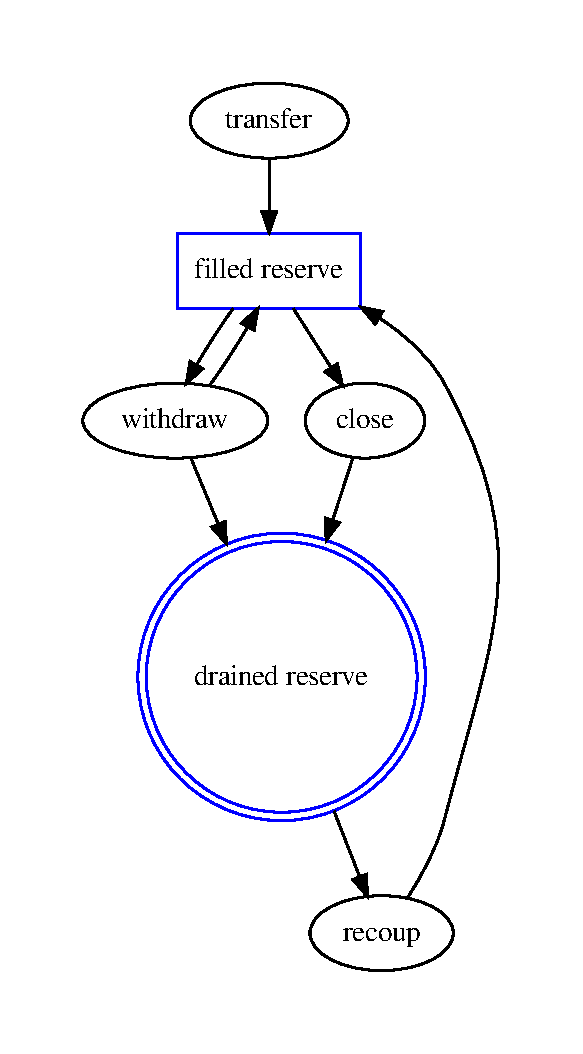
\includegraphics{taler/reserve.pdf}
  \end{center}
  \caption{State machine of a reserve.}
  \label{fig:reserve:states}
\end{figure}

Instead of requiring the customer to manually generate reserve key pairs and
copy them onto a wire transfer form, banks can offer tight integration with the
GNU Taler wallet software.  In this scenario, the bank's website or banking app
provides a ``withdraw to GNU Taler wallet'' action.  After selecting this
action, the user is asked to choose the amount to withdraw from their bank
account into the wallet.  The bank then instructs the GNU Taler wallet software
to create record of the corresponding reserve; this request contains the anticipated amount, the
reserve key pair and the URL of the exchange to be used.  When invoked by the
bank, the wallet asks the customer to select an exchange and to confirm the
reserve creation.  The exchange chosen by the customer must support the wire
transfer method used by the bank, which will be automatically checked by the
wallet.  Typically, an exchange is already selected by default, as banks can
suggest a default exchange provider to the wallet, and additionally wallets
have a pre-defined list of trusted exchange providers.  Subsequently, the wallet
hands the reserve public key and the bank account information of the selected
exchange back to the bank.  The bank---typically after asking for a second authentication
factor from the customer---will then trigger a wire transfer to the exchange with
the information obtained from the wallet.

When the customer's bank does not offer tight integration with GNU Taler, the
customer can still manually instruct their wallet to create a reserve.  The public
key must then be included in a bank transaction to the exchange.  When the
customer's banking app supports pre-filling wire transfer details from a URL or
a QR code, the wallet can generate such a URL or QR code that includes the
pre-filled bank account details of the exchange as well as the reserve public
key.  The customer clicks on this link or scans the QR code to invoke their
banking app with pre-filled transaction details.  Since there currently is no
standardized format for pre-filled wire transfer details, we are proposing the
\texttt{payto://} URI format explained in
Section~\ref{implementation:wire-method-identifiers}, currently under review
for acceptance as an IETF Internet Standard.


% FIXME: withdrawal strategy, coin selection

\subsection{Coins and Denominations}

Unlike plain Chaumian e-cash, where a coin just contains a serial number, a
\emph{coin} in Taler is a public/private key pair where the private key is only
known to the owner of the coin.

A coin derives its financial value from a blind signature on the coin's
public key. The exchange has multiple \emph{denomination key} pairs available
for blind-signing coins of different financial values.  Other approaches for representing
different denominations are discussed in Section~\ref{design:related-different-denominations}.

Denomination keys have an expiration date, before which any coins signed with
it must be spent or exchanged into newer coins using the refresh protocol
explained in Section \ref{sec:design-refresh}.  This allows the exchange to
eventually discard records of old transactions, thus limiting the records that
the exchange must retain and search to detect double-spending attempts.  If a
denomination's private key were to be compromised, the exchange can detect this
once more coins are redeemed than the total that was signed into existence
using that denomination key.  Should such an incident occur, the exchange can allow authentic
customers to redeem their unspent coins that were signed with the compromised
private key, while refusing further deposits involving coins signed by the
compromised denomination key (see Section~\ref{sec:revocation-recoup}).  As a result, the
financial damage of losing a private signing key is limited to at most the
amount originally signed with that key, and denomination key rotation can be
used to bound that risk.

To prevent the exchange from deanonymizing users by signing each coin with a
fresh denomination key, exchanges publicly announce their denomination keys
in advance with validity periods that imply sufficiently strong anonymity sets.
These announcements are expected to be signed with an offline long-term
private \emph{master signing key} of the exchange and the auditor.
Customers should obtain these announcements using an anonymous
communication channel.

After a coin is issued, the customer is the only entity that knows the
private key of the coin, making them the \emph{owner} of the coin.  Due
to the use of blind signatures, the exchange does not learn the
public key during the withdrawal process.  If the private key is
shared with others, they become co-owners of the coin.  Knowledge of
the private key of the coin and the signature over the coin's public
key by an exchange's denomination key enables spending the
coin.

\subsection{Partial Spending and Unlinkable Change}

Customers are not required to have exact change ready when making a payment.
In fact, it should be encouraged to withdraw a larger amount of e-cash
beforehand, as this blurs the correlation between the non-anonymous withdrawal
event and the anonymous spending event, increasing the anonymity set.

A customer spends a coin at a merchant by cryptographically signing a
\emph{deposit permission} with the coin's private key.  A deposit permission
contains the hash of the \emph{contract terms}, i.e., the details of the
purchase agreement between the customer and merchant. Coins can be
\emph{partially} spent, and a deposit permission specifies the fraction of the
coin's value to be paid to the merchant. As digital coins are trivial to copy,
the merchant must immediately deposit them with the exchange, in order to get a
deposit confirmation or an error that indicates double spending.

When a coin is used in a completed or attempted/aborted payment, the coin's
public key is revealed to the merchant/exchange, and further payments with the
remaining amount would be linkable to the first spending event.  To obtain
unlinkable change for a partially spent (or otherwise revealed coin), GNU
Taler introduces the \emph{refresh protocol}, which consists of three steps:
\emph{melt}, \emph{reveal} and \emph{link}.  The refresh protocol allows the
customer to obtain new coins for the remaining amount on a coin.  The old coin
is marked as spent after it has been melted, while the reveal step generates
the fresh coins.  Using blind signatures to withdraw the refreshed coins makes
them unlinkable from the old coin.

% FIXME: talk about logarithmic time, simulation

\subsection{Refreshing and Taxability}\label{sec:design-refresh}
% FIXME:  maybe put section on how to avoid withdraw loophole here!
One goal of GNU Taler is to make merchants' income transparent to state auditors,
so that income can be taxed appropriately.  Naively implemented, however, a simple
refresh protocol could be used to evade taxes:  the payee of an untaxed
transaction would generate the private keys for the coins that result from
refreshing a (partially spent) old coin, and send the corresponding public keys
to the payer.  The payer would execute the refresh protocol, provide the
payee's coin public keys for blind signing, and provide the signatures to the
payee, who would now have exclusive control over the coins.

To remedy this, the refresh protocol introduces a \emph{link threat}: coins are
refreshed in such a way that the owner of the old coin can always obtain the
private key and exchange's signature on the new coins resulting from refreshes,
using a separate \emph{linking protocol}.  This introduces a threat to
merchants that try to obtain untaxed income.  Until the coins are finally
deposited at the exchange, the customer can always re-gain ownership of them
and could deposit them before the merchant gets a chance to do so.  This
disincentivizes the circulation of unreported income among untrusted parties in
the system.

In our implementation of the refresh and linking protocols, there is a
non-negligible success chance ($\frac{1}{\kappa}$, depending on system parameter
$\kappa$, typically $\ge 3$) for attempts to cheat during the refresh protocol,
resulting in refreshed coins that cannot be recovered from the old coin via the
linking protocol.  Cheating during refresh, however, is still not
\emph{profitable}, as an unsuccessful attempt results in completely losing the
amount that was intended to be refreshed.

% FIXME:  mention that we don't want to use DRM/HSMs for this

For purposes of anti-money-laundering and taxation, a more detailed audit of
the merchant's transactions can be desirable.  A government tax authority can
request the merchant to reveal the business agreement details that match the
contract terms hash recorded with the exchange.  If a merchant is not able to
provide theses values, they can be subjected to financial penalties by the
state in relation to the amount transferred by the traditional currency
transfer.

\subsection{Transactions vs. Sharing}

Sharing---in contrast to a transaction---happens when mutually trusted parties
simultaneously have access to the private keys and signatures on coins.
Sharing is not considered a transaction, as subsequently both parties have equal control
over the funds.  A useful application for sharing are peer-to-peer payments
between mutually trusting parties, such as families and friends.

\subsection{Aggregation}

For each payment, the merchant can specify a deadline before which the exchange
must issue a wire transfer to the merchant's bank account.  Before this
deadline occurs, multiple payments from deposited coins to the same merchant
can be \emph{aggregated} into one bigger payment.  This reduces transaction
costs from underlying banking systems, which often charge a fixed fee per
transaction.  To incentivize merchants to choose a longer wire transfer
deadline, the exchange can charge the merchant a fee per aggregated wire
transfer.

Figure~\ref{fig:deposit:states} illustrates the state machine for processing
deposits.  Long-terms states are shown in boxes, while actions are in circles.
The final state is in a double-circle.  Dashed arrows show transitions based
on timing and not external actions. A deposit is first {\em created} when a
wallet makes a payment.  A deposit comes with a {\em refund deadline}, and the
wire transfer must not happen before that deadline. Once the refund deadline
has passed, the deposit becomes {\em ready}.  Even if a deposit is ready, it
is not automatically wired. In fact, deposits may still be {\em refunded} in
this state.  A refund may be full (resulting in the deposit being {\em done})
or partial, in which case the remaining value is left in the same deposit
state. A deposit comes with a second deadline, the {\em wire deadline}. Once
that deadline has passed, the deposit is {\em due} and must be {\em
  aggregated}.  Aggregation combines {\bf all} deposits that are {\em due},
{\em tiny} or {\em ready} into one wire transfer.  However, the amount of even
an aggregated deposit may be too small to be executed by the banking
system. In this case, the deposit transitions into the special state {\em
  tiny} until the aggregated amount meets the amount threshold.  Once
aggregated, the deposits are {\em done}.  A wire transfer is first prepared
and then {\em pending}. The transfer is {\em finished} once the bank has
confirmed the {\em transfer}.

\begin{figure}
  \begin{center}
    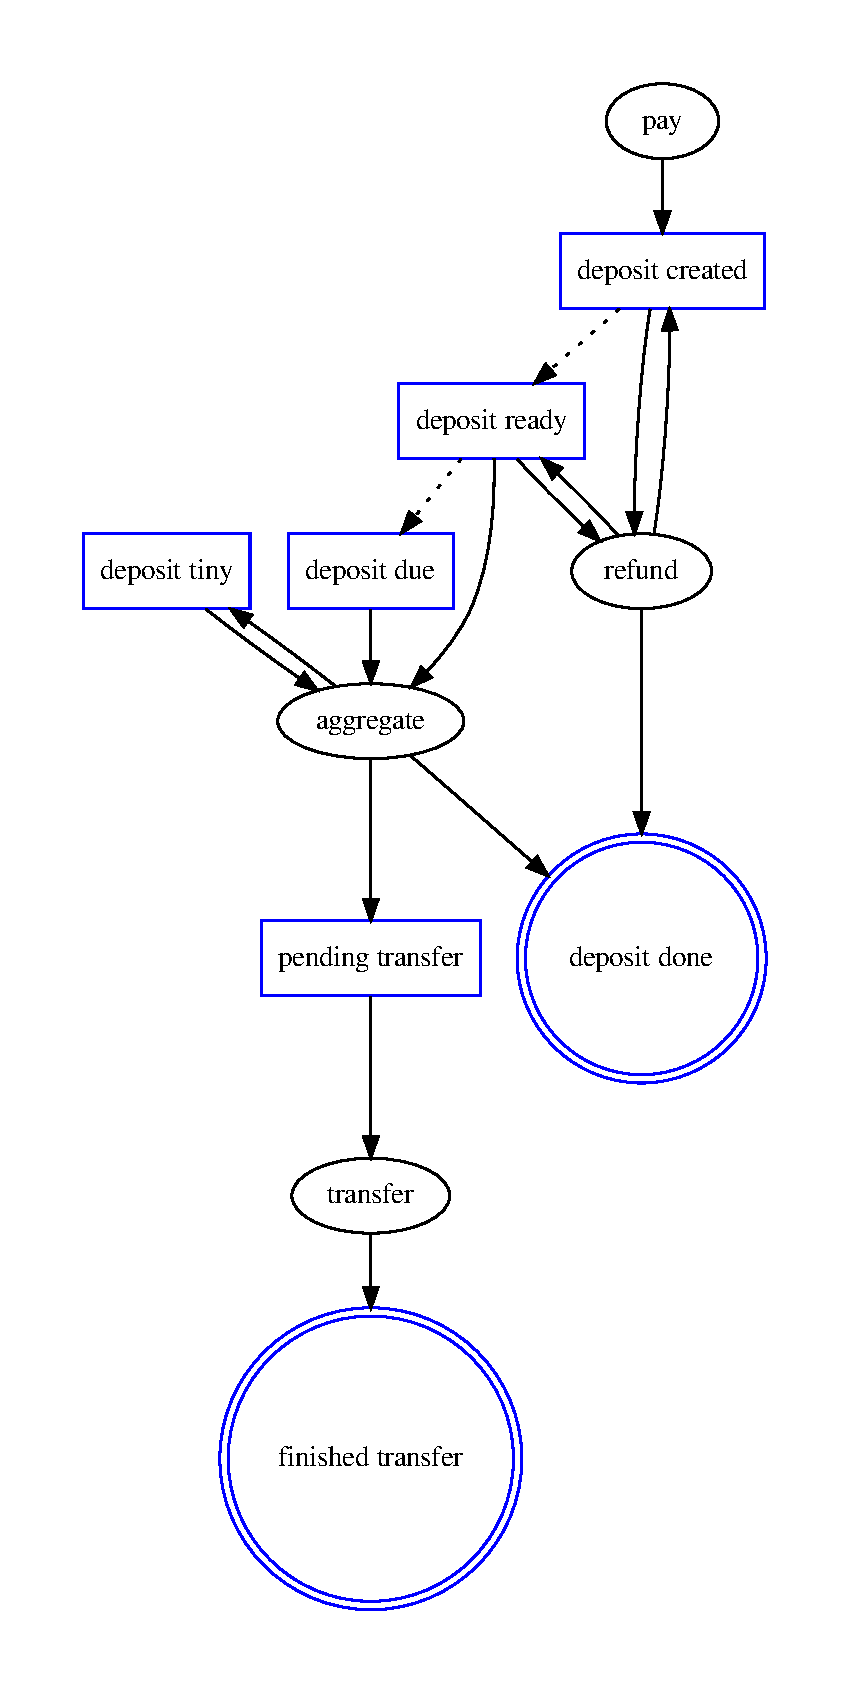
\includegraphics[scale=0.8]{taler/deposit.pdf}
  \end{center}
  \caption{State machine of a deposit.}
  \label{fig:deposit:states}
\end{figure}


\subsection{Refunds}

The aggregation period also opens the opportunity for cheap \emph{refunds}.  If
a customer is not happy with their product, the merchant can instruct the
exchange to give the customer a refund before the wire transfer deadline has
occurred.  This effectively ``undoes'' the deposit of the coin, and restores the
available amount left on it.  The refresh protocol is then used by the customer
on the coins involved in a refund, so that payments remain unlinkable.

% FIXME: mention EU customer laws / 14 weeks?

\subsection{Fees}

In order to subsidize the operation of the exchange and enable a sustainable
business model, the exchange can charge fees for most operations.  For
withdrawal, refreshing, deposit and refunds, the fee is dependent on the denomination,
as different denominations might have different key sizes, security and storage
requirements.

Most payment systems hide fees from the customer by putting them to the merchant.
This is also possible with Taler.  As different exchanges (and denominations)
can charge different fees, the merchant can specify a maximum amount of fees it
is willing to cover.  Fees exceeding this amount must be explicitly paid by the
customer.

Another consideration for fees is the prevention of denial-of-service attacks.
To make ``useless'' operations, such as repeated refreshing on coins
(causing the exchange to use relatively expensive storage), unattractive to an
adversary, these operations must charge a fee.  Again, for every refresh
following a payment, the merchant can cover the costs up to a limit set by the
merchant, effectively hiding the fees from the customer.

Yet another type of fee are the \emph{wire transfer fees}, which are charged
by the exchange for every wire transfer to a merchant in order to compensate for
the cost of making a transaction in the underlying bank system.  The wire
transfer fees encourage merchants to choose longer aggregation periods, as the
fee is charged per transaction and independant of the amount.

Merchants can also specify the maximum wire fee they are willing to cover for
customers, along with an \emph{amortization rate} for the wire fees.  In case
the wire fees for a payment exceed the merchant's chosen maximum, the customer
must additionally pay the excess fee divided by the amortization rate.  The
merchant should set amortization rate to the expected number of transactions
per wire transfer aggregation window.  This allows the merchant to adjust
the total expected amount that it needs to pay for wire fees.


\subsection{The Withdraw Loophole and Tipping}\label{taler:design:tipping}

The withdraw protocol can be (ab)used to illicitly transfer money, when the
receiver generates the coin's secret key, and gives the public key to the party
executing the withdraw protocol.  We call this the ``withdraw loophole''.  This
is only possible for one ``hop'', as money can still not circulate among
mutually distrusted parties, due to the properties of the refresh protocol.

A ``benevolent'' use of the withdraw loophole is \emph{tipping}, where merchants give
small rewards to customers (for example, for filling out a survey or installing
an application), without any contractual obligations or digitally signed
agreement.

% FIXME:  argue that this can't be done on scale for money laundering

\subsubsection{Fixing the Withdraw Loophole}\label{taler:design:fixing-withdraw-loophole}

In order to discourage the usage of the withdraw loophole for untaxed payments,
the following approach would be possible:  Normal withdraw operations and
unregistered reserves are disabled, except for special tip reserves that are
registered by the merchant as part of a tipping campaign.  Customers are
required to pre-register at the exchange and obtain a special withdraw key pair
against a small safety deposit.  Customer obtain new coins via a refresh
operation from the withdraw key to a new coin.  If customers want to abuse
Taler for untaxed payments, they either need to risk losing money by lying
during the execution of the refresh protocol, or share their reserve private
key with the payee.  In order to discourage the latter, the exchanges gives the
safety deposit to the first participant who reports the corresponding private
key as being used in an illicit transaction, and requires a new safety deposit
before the customer is allowed to withdraw again.

However since the withdraw loophole allows only one additional ``payment'' (without any
cryptographic evidence that can be used in disputes) before the coin must be deposited,
these additional mitigations might not even be justified considering their additional cost.


\section{Auditing}

The auditor is a component of GNU Taler which would typically be deployed by a
financial regulator, fulfilling the following functionality:

\begin{itemize}
  \item It regularly examines the exchange's database and
    bank transaction history to detect discrepancies.
  \item It accepts samples of certain protocol responses that merchants
    received from an audited exchange, to verify that what the exchange signed
    corresponds to what it stored in its database.
  \item It certifies exchanges that fulfill the operational and financial requirements
    demanded by regulators.
  \item It regularly runs anonymous checks to ensure that the required protocol
    endpoints of the exchange are available.
  \item In some deployment scenarios, merchants need to pre-register with exchanges to fulfill know-your-customer (KYC) requirements.
    The auditor provides a list of certified exchanges to merchants,
    to which the merchant then can automatically KYC-register.
  \item It provides customers with an interface to submit cryptographic proof that an exchange
    misbehaved.  If a customer claims that the exchange denies service, it can execute a request on
    behalf of the customer.
\end{itemize}

%An exchange operator would typically run their own instance of the auditor software,
%to ensure correct operation.

% FIXME: live auditing

% FIXME: discuss indian merchant scenario

\subsection{Exchange Compromise Modes}

The exchange is an attractive target for hackers and insider threats.  We now
discuss different ways that the exchange can be compromised, how to reduce the
likelihood of such a compromise, and how to detect and react to such an event
if it happens.

\subsubsection{Compromise of Denomination Keys and Revocation}\label{sec:revocation-recoup}

When a denomination key pair is compromised, an attacker can ``print money'' by
using it to sign coins of that denomination.  An exchange (or its auditor) can
detect this when the number of deposits for a certain denomination exceed the
number of withdrawals for that same denomination.

We allow the exchange to revoke denomination keys, and wallets periodically
check for such revocations.  We call a coin of a revoked denomination a revoked
coin.  If a denomination key has been revoked, the wallets use the
\emph{recoup} protocol to recover funds from coins of revoked denominations.
Once a denomination is revoked, new coins of this denomination can't be
withdrawn or used as the target denomination for a refresh operation. A revoked
coin cannot be spent, and can only be refreshed if its public key was recorded
in the exchange's database (as spending/refresh operations) before it was
revoked.

The following cases are possible for recoup:
\begin{enumerate}
  \item The revoked coin has never been seen by the exchange before, but the
    customer can prove via a withdraw protocol transcript and blinding factor
    that the coin resulted from a legitimate withdrawal from a reserve.  In
    this case, the exchange credits the reserve that was used to withdraw the
    coin with the value of the revoked coin.
  \item The coin has been partially spent.  In this case, the exchange allows
    the remaining amount on the coin to be refreshed into fresh coins of
    non-revoked denominations.
  \item The revoked coin $C_R$ has never been seen by the exchange before, was
    obtained via the refresh protocol, and the exchange has an existing record
    of either a deposit or refresh for the ancestor coin $C_A$ that was
    refreshed into the revoked coin $C_R$. If the customer can prove this by
    showing a corresponding refresh protocol transcript and blinding factors, the exchange credits
    the remaining value of $C_R$ on $C_A$.  It is explicitly permitted for $C_A$
    to be revoked as well.  The customer can then obtain back their funds by
    refreshing $C_A$.
\end{enumerate}

These rules limit the maximum financial damage that the exchange can incur from
a compromised denomination key $D$ to $2nv$, with $n$ being the
maximum number of $D$-coins simultaneously in circulation and $v$ the financial
value of a single $D$-coin.  Say denomination $D$ was withdrawn by
legitimate users $n$ times.  As soon as the exchange sees more
than $n$ pairwise different $D$-coins, it must immediately
revoke $D$.  An attacker can thus at most gain $nv$ by either
refreshing into other non-revoked denominations or spending the forged $D$-coins.
The legitimate users can then request a recoup for their coins, resulting in
a total financial damage of at most $2nv$.

With one rare exception, the recoup protocol does not negatively impact the
anonymity of customers.  We show this by looking at the three different cases
for recoup on a revoked coin.  Specifically, in case (1), the coin obtained
from the credited reserve is blindly signed, in case (2) the refresh protocol
guarantees unlinkability of the non-revoked change, and in case (3) the revoked
coin $C_R$ is assumed to be fresh.  If $C_R$ from case (3) has been seen by a
merchant before in an aborted/unfinished transaction, this transaction would be
linkable to transactions on $C_A$.  Thus, anonymity is not preserved when an
aborted transaction coincides with revoked denomination, which should be rare
in practice.

Unlike most other operations, the
recoup protocol does not incur any transaction fees. The primary use of the
protocol is to limit the financial loss in cases where an audit reveals that
the exchange's private keys were compromised, and to automatically pay back
balances held in a customers' wallet if an exchange ever goes out of business.

To limit the damage of a compromise, the exchange can employ a hardware
security module that contains the denomination secret keys, and is
pre-programmed with a limit on the number of signatures it can produce.  This
might be mandated by certain auditors, who will also audit the operational
security of an exchange as part of the certification process.



\subsubsection{Compromise of Signing Keys}

When a signing key is compromised, the attacker can pretend to be a
merchant and forge deposit confirmations.  To forge a deposit
confirmation, the attacker also needs to get a customer to sign a
contract from the adversary (which should include the adversary's
banking details) with a valid coin.  The attack here is that the
customer is allowed to have spent the coin already. Thus, a deposit of
the resulting deposit permission would result in a rejection from the
exchange due to double spending.  By forging the deposit confirmation
using the compromised signing key, the attacker can thus claim in
court that they properly deposited the coin first and demand payment
from the exchange.

We note that indeed an evil exchange could simply fail to record
deposit permissions in its database and then fail to execute them.
Thus, given a merchant presenting a deposit confirmation, we need
a way to establish whether this is a case of an evil exchange that
should be compelled to pay, or a case of a compromised signing key
and where payouts (and thus financial damage to the exchange)
can legitimately be limited.

To limit the financial damage of a compromised signing key, merchants
must be required to work with auditors to perform a
\emph{probabilistic deposit auditing} of the exchange.  Here, the goal
is to help detect the compromise of a signing key by making sure that
the exchange does indeed properly record deposit confirmations.
However, double-checking with the auditor if every deposit
confirmation is recorded in the exchange's database would be too
expensive and time-consuming.  Fortunately, a probabilistic method
where merchants only send a small fraction of their deposit
confirmations to the auditor suffices.  Then, if the auditor sees a
deposit confirmation that is not recorded in the exchange's database
(possibly after performing the next synchronization with the
exchange's database), it signals the exchange that the signing key has
been compromised.

At this point, the signing key must be revoked and the exchange will
be required to investigate the security of its systems and address the
issue before resuming normal operations.
%
%If the exchange had separate short-term signing keys just for signing deposit
%confirmations, it could also employ hardware security modules with a counter,
%and check if the value of the counter matches matches the deposit confirmations
%recorded in the database.

Still, at this point various actors (including the attacker) could still
step forward with deposit confirmations signed by the revoked key and
claim that the exchange owes them for their deposits.  Simply revoking
a signing key cannot lift the exchange's payment obligations, and the
attacker could have signed an unlimited number of such deposit confirmations
with the compromised key.  However, in contrast to honest merchants, the
attacker will not have participated {\em proportionally} in the auditor's
probabilistic deposit auditing scheme for those deposit confirmations:
in that case, the key compromise would have been detected and the key
revoked.

The exchange must still pay all deposit permissions it signed for
coins that were not double-spent.  However, for all coins where
multiple merchants claim that they have a deposit confirmation, the
exchange will pay the merchants proportionate to the fraction of the
coins that they reported to the auditor as part of probabilistic
deposit auditing.  For example, if 1\% of deposits must be reported to
the auditor according to the protocol, a merchant might be paid at
most say 100+X times the number of reported deposits where $X>0$
serves to ensure proper payout despite the probabilistic nature of the
reporting.  As a result, honest merchants have an {\em incentive} to
correctly report the deposit confirmations to the auditor.

Given this scheme, the attacker can only report a small number of
deposit confirmations to the auditor before triggering the signing key
compromise detection.  Suppose again that 1\% of deposit confirmations
are reported by honest merchants, then the attacker can only expect to
submit 100 deposit permissions created by the compromised signing key
before being detected.  The attacker's expected financial benefit from
the key compromise would then be the value of $(100+X) \cdot 100$
deposit permissions.

Thus, the financial benefit to the attacker can be limited by
probabilistic deposit auditing, and honest merchants have proper
incentives to participate in the process.

\subsubsection{Compromise of the Database}

If an adversary would be able to modify the exchange, this would be detected
rather quickly by the auditor, provided that the database has appropriate
integrity mechanisms.  An attacker could also prevent database updates to block
the recording of spend operations, and then double spend.  This is effectively
equivalent to the compromise of signing keys, and can be detected with the same
strategies.

\subsubsection{Compromise of the Master Key}

If the master key was compromised, an attacker could de-anonymize customers by
announcing different sets of denomination keys to each of them.  If the
exchange was audited, this would be detected quickly, as these denominations
will not be signed by auditors.

\subsection{Cryptographic Proof}

We use the term ``proof'' in many places as the protocol provides cryptographic
proofs of which parties behave correctly or incorrectly. However,
as~\cite{fc2014murdoch} point out, in practice financial systems need to
provide evidence that holds up in courts.  Taler's implementation is designed
to export evidence and upholds the core principles described
in~\cite{fc2014murdoch}.  In particular, in providing the cryptographic proofs
as evidence none of the participants have to disclose their core secrets.

\subsection{Perfect Crime Scenarios}\label{sec:design:blackmailing}

GNU Taler can be slightly modified to thwart blackmailing or kidnapping
attempts by criminals who intend to use the anonymity properties of the system
and demand to be paid ransom in anonymous e-cash.

Our modification incurs a slight penalty on the latency for customers during normal use and
requires slightly more data to be stored in the exchange's database, and thus
should only be used in deployments where resistance against perfect crime
scenarios is necessary.  A payment system for a school cafeteria likely does
not need these extra measures.

The following modifications are made:
\begin{enumerate}
  \item Coins can now only be used in either a transaction or in a refresh operations, not a mix of both.
    Effectively, the customer's wallet then needs to use the refresh protocol to prepare exact change
    before a transaction is made, and that transaction is made with exact change.

    This change is necessary to preserve anonymity in face of the second modification, but increases
    storage requirements and latency.
  \item The recoup protocol is changed so that a coin obtained
    via refreshing must be recovered differently when revoked: to recover a revoked coin
    obtained via refreshing, the customer needs to show the transcripts for the
    chain of all refresh operations and the initial withdrawal operation
    (including the blinding factor).  Refreshes on revoked coins are not
    allowed anymore.
\end{enumerate}

After an attacker has been paid ransom, the exchange simply revokes all currently offered denominations
and registers a new set of denomination with the auditor.
Reserves used to pay the attacker are marked as blocked in the exchange's
database.  Normal users can use the recoup protocol to obtain back the money
they've previously had in revoked denominations.  The attacker can try to
recover funds via the (now modified) recoup protocol, but this attempt will
not be successful, as the initial reserve is blocked.  The criminal could also
try to spend the e-cash anonymously before it is revoked, but this is likely
difficult for large amounts, and furthermore due to income transparency all
transactions made between the payment of the ransom and the revocation can be
traced back to merchants that might be complicit in laundering the ransom
payment.

Honest customers can always use the recoup protocol to transfer the funds to
the initial reserve.  Due to modification (1), unlinkability of transactions is
not affected, as only coins that were purely used for refreshing can now be
correlated.

We believe that our approach is more practical than the approaches based on
tracing, since in a scheme with tracing, the attacker can always ask for a
plain blind signature.  With our approach, the attacker will always lose funds
that they cannot immediately spend.  Unfortunately our approach is limited to a
kidnapping scenario, and not applicable in those blackmail scenarios where the
attacker can do damage after they find out that their funds have been erased.

\subsection{Summary}

Figure~\ref{fig:coin:states} illustrates the overall state machine for processing
coins.  Long-terms states are shown in boxes, while actions are in circles.
The final state is in a double-circle.  Dashed arrows show transitions based
on timing and not external actions. The red arrow shows an action that is
allowed by the exchange but should never be done by wallets as it would
break unlinkability.

A coin begins as an unsigned {\em planchet}, which is either signed as part of
the {\em withdraw} protocol or the refresh protocol. The most common scenario
is that the {\em fresh coin} is {\em deposited}. This payment creates a
deposit (see Figure~\ref{fig:deposit:states}) and either a {\em dirty coin}
(if the payment was for a fraction of the coin's value) or a {\em spent coin}.
A spent coin can be {\em refunded} by the merchant, creating a {\em dirty
  coin}. Once the exchange has aggregated a coin and wired the amount to the
merchant, a coin can no longer be refunded.

A {\em fresh coin} may also be subject to key {\em revocation}, at which point
the wallet ends up with a {\em revoked coin}.  At this point, the wallet can
use the {\em recoup} protocol to recover the value of the coin.  If the coin
originated from a {\em withdraw} operation, the value is added back into the
reserve, which is {\em filled} in the process (see
Figure~\ref{fig:reserve:states}).  If the coin originated from the {\em
  refresh} operation, this results in the old coin turning into a {\em zombie
  coin}, which can be refreshed again.

Dirty coins and fresh coins can be {\em melted}.  Dirty coins should always be
melted automatically by the wallet as soon as possible as this is the only
good way to use them while preserving unlinkability.  A wallet should also
automatically {\em melt} any {\em fresh coins} that are in danger of their
denomination key nearing its (deposit) {\em expiration} time. If a wallet
fails to do so, coins may {\em expire}, resulting in a loss for the coin's
owner.  Dirty coins can also expire. In practice, this happens if the melt fee
exceeds the residual value of the dirty coin.  To {\em melt} a coin, the
wallet must commit to one or more {\em planchets} and then demonstrate honesty
when the committment made for the {\em refresh session} is checked during the
{\em reveal} step. If the wallet was honest, {\em reveal} yields {\em fresh
  coins}.

\begin{figure}
  \begin{center}
    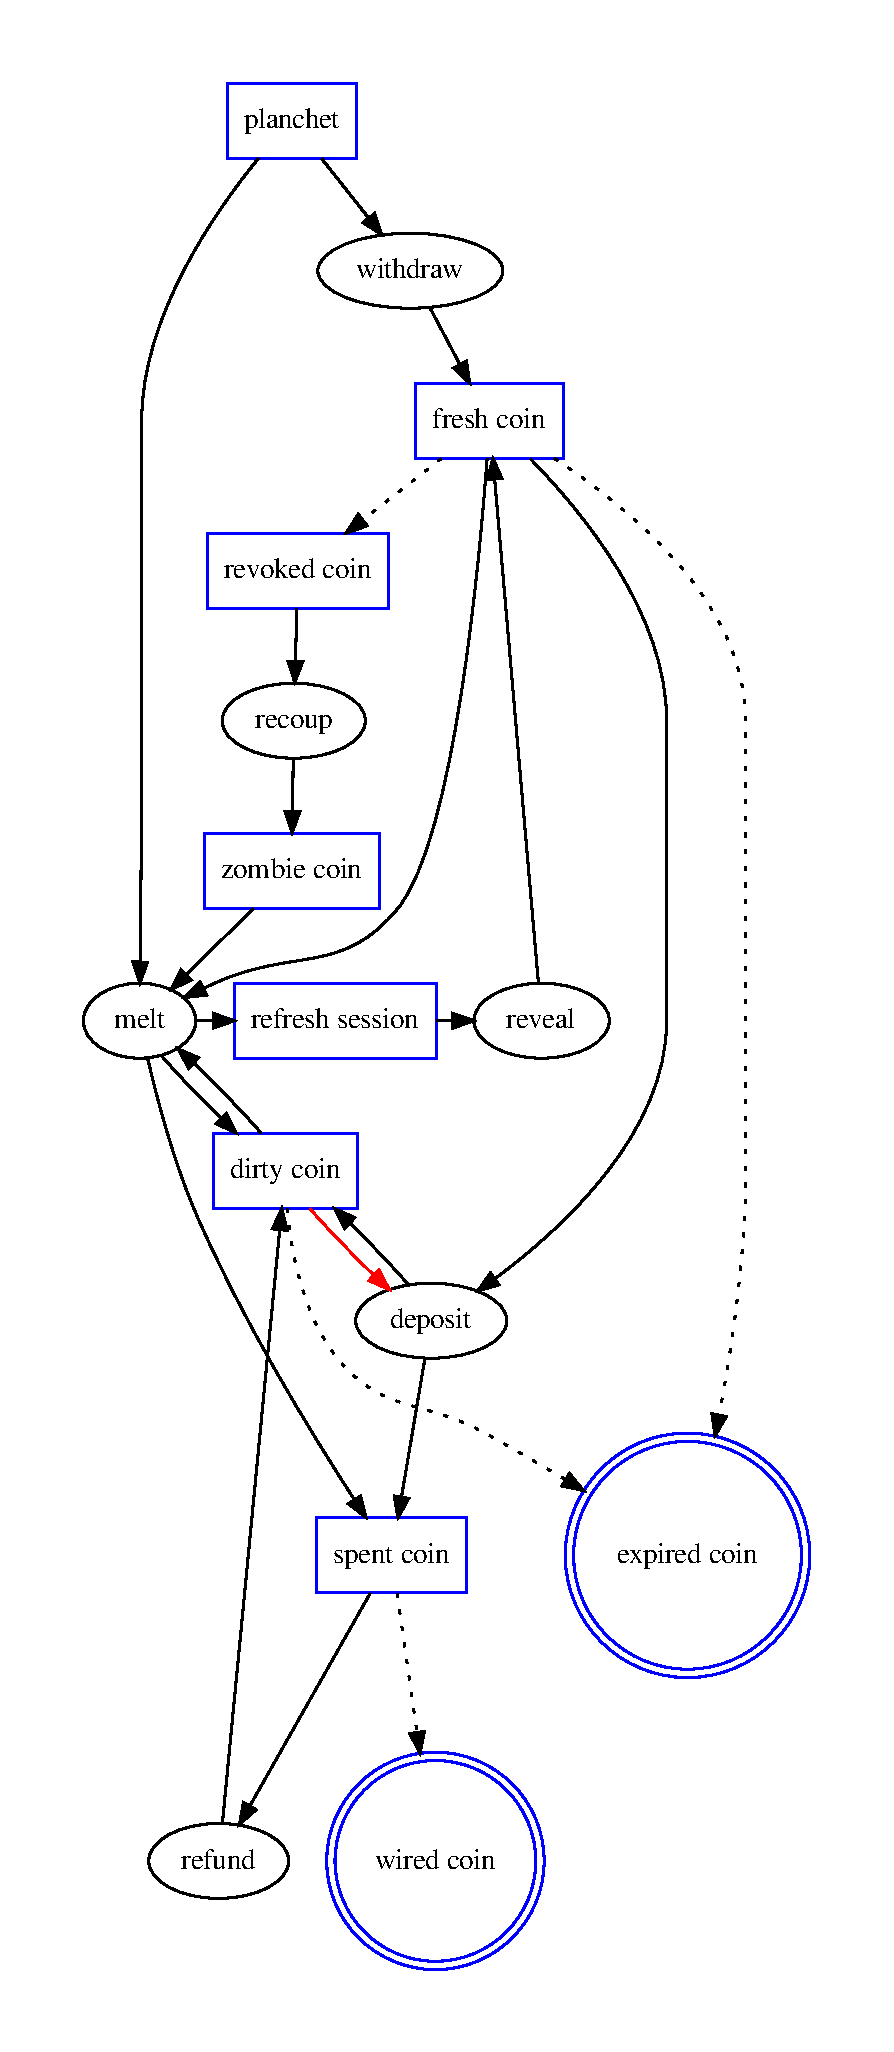
\includegraphics[scale=0.65]{taler/coin.pdf}
  \end{center}
  \caption{State machine of a coin.}
  \label{fig:coin:states}
\end{figure}





\section{Related Work}
% FIXME: Stuff to review/include:
% Blindly Signed Contracts: Anonymous On-Blockchain and Off-Blockchain Bitcoin Transactions
% zcash taxability stuff

\subsection{Anonymous E-Cash}\label{sec:related-work:e-cash}

Chaum's seminal paper \cite{chaum1983blind} introduced blind signatures and
demonstrated how to use them for online e-cash.  Later work
\cite{chaum1989efficient,chaum1990untraceable} introduced offline spending, where additional
information is encoded into coins in such a way that double spending reveals
the culprit's identity.

Okamoto \cite{okamoto1995efficient} introduced the first efficient offline
e-cash scheme with divisibility, a feature that allows a single coin to be
spent in parts.  With Okamoto's protocol, different spending operations that
used parts of the same coin were linkable.  An unlinkable version of
divisible e-cash was first presented by Canard~\cite{canard2007divisible}.

Camenisch's compact e-cash \cite{camenisch2005compact} allows wallets with $2^\ell$ coins to be stored
and withdrawn with storage, computation and computational costs in $\mathcal{O}(\ell)$.
Each coin in the wallet, however, still needs to be spent separately.

The protocol that can currently be considered the state-of-the-art for efficient
offline e-cash was introduced by Pointcheval et al. \cite{pointcheval2017cut}.
It allows constant-time withdrawal of a divisible coin, and constant-time
spending of a continuous ``chunk'' of a coin.  While the pre-determined number
of divisions of a coin is independent from the storage, bandwidth and
computational complexity of the wallet, the exchange needs to check for
double-spending at the finest granularity.  Thus, highly divisible coins incur
large storage and computational costs for the exchange.

An e-cash system with multiple denominations with different financial values
was proposed by Canard and Gouget~\cite{canard2006handy} in the context of a divisible
coupon system.

One of the earliest mentions of an explicit change protocol can be found in
\cite{brickell1995trustee}.  Ian Goldberg's HINDE system is another design that
allows the merchant to provide change, but the mechanism could be abused to
hide income from taxation.\footnote{Description based on personal
communication. HINDE was never published, but supposedly publicly discussed at
Financial Crypto '98.}  Another online e-cash protocol with change was proposed
by Tracz \cite{tracz2001fair}.  The use of an anonymous change protocol (called
a ``refund'' in their context) for fractional payments has also been suggested
for a public transit fees payment system \cite{rupp2013p4r}.  Change protocols
for offline e-cash were recently proposed \cite{batten2018offline}.  To the
best of our knowledge, no change protocol with protections against tax evasion
has been proposed so far, and all change protocols suggested so far can be
(ab)used to make a payment into another wallet.

Transferable e-cash allows the transfer of funds between customers without
using the exchange as in intermediary \cite{fuchsbauer2009transferable}.

Chaum also proposed wallets with observers \cite{chaum1992wallet} as a
mechanism against double spending.  The observer is a tamper-proof hardware
security module that prevents double-spending, while at the same time being
unable to de-anonymize the user.

Various works propose mechanisms to selectively de-anonymize customers or
transactions that are suspected of criminal activities
\cite{stadler1995fair,davida1997anonymity}.  Another approach suspends
customers that were involved in a particular transaction, while keeping the
customer anonymous \cite{au2011electronic}.

One of the first formal treatments of the provable security of e-cash was given
in \cite{damgaard2007proof}.  The first complete security definition for blind
signatures was given by Pointcheval \cite{pointcheval1996provably} and applied
to RSA signatures later \cite{pointcheval2000security}.  While the security
proof of RSA signatures requires the random oracle model, many blind signature
schemes are provably secure in the standard model
\cite{izabachene2013divisible,pointcheval2017cut}.  While most literature
provides only ``human-verified'' security arguments, the security of a simple
e-cash scheme has been successfully modeled in
ProVerif~\cite{dreier2015formal}, albeit only in the symbolic model.

\subsubsection{Implementations}
DigiCash was the first commercial implementation of Chaum's e-cash.  It
ultimately failed to be widely adopted, and the company filed for bankruptcy in
1998.  Some details of the implementation are available
\cite{schoenmakers1997security}.  In addition to Chaum's infamously paranoid
management style \cite{next1999digicash}, reasons for DigiCash's failure could
have been the following:

\begin{itemize}
 \item DigiCash did not allow account-less operations.  To use DigiCash,
   customers had to sign up with a bank that natively supports DigiCash.
 \item DigiCash did not support change or partial spending, negating a lot of
   the convenience and security of e-cash by requiring frequent withdrawals
    from the customer's bank account.
 \item The technology used by DigiCash was protected by patents,
   which stifled innovation from competitors.
 \item Chaum's published design does not clearly limit the financial damage an
   exchange might suffer from the disclosure of its private online signing key.
\end{itemize}

To our knowledge, the only publicly available effort to implement anonymous
e-cash is Opencoin~\cite{dent2008extensions}.  However, Opencoin is neither
actively developed nor used, and it is not clear to what degree the
implementation is even complete.  Only a partial description of the Opencoin
protocol is available to date.


\subsubsection{Representing Denominations}\label{design:related-different-denominations}

For GNU Taler, we chose to represent denominations of different values by a
different public key for every denomination, together with a mapping from
public key to financial value and auxiliary information about fees and
expiration dates.  This approach has the advantage that coins of higher denominations
can be signed by denominations with a larger key size.

Schoenmakers~\cite{schoenmakers1997security} proposes an optimized
implementation of multiple denomination that specifically works with RSA keys,
which encodes the denomination in the public exponent $e$ of the RSA public
key, while the modulus $N$ stays the same for all denominations.  An advantage
of this scheme is the reduced size of the public keys for a set of
denominations.  As this encoding is specific to RSA, it would be difficult for
future versions of this protocol to switch to different blind signature
primitives.  More importantly, factoring $N$ would lead to a compromise of all
denominations instead of just one.

Partially blind signatures can be used to represent multiple denominations
by blindly signing the coin's serial number and including the financial value of the coin
in the common information seen by both the signer and signee \cite{abe2000provably}.

The compact e-cash scheme of Märtens~\cite{maertens2015practical} allows
constant-time withdrawal of wallets with an arbitrary number of coins, as long
as the number of coins is smaller than some system parameter.  This approach
effectively dispenses with the need to have different denominations.


\subsubsection{Comparison}

\newcommand\YES{\ding{51}} % {\checkmark}
\newcommand\NO{\ding{55}}

\newcommand*\rot{\multicolumn{1}{R{45}{1em}}}% no optional argument here, please!
%\newcommand*\rot{}% no optional argument here, please!


\newcolumntype{H}{>{\setbox0=\hbox\bgroup}c<{\egroup}@{}}

\newcolumntype{R}[2]{%
    >{\adjustbox{angle=#1,lap=\width-(#2)}\bgroup}%
    l%
    <{\egroup}%
}

{\footnotesize
\begin{tabular}{r|ccccccccccc}
&
\rot{Year} &
\rot{Implementation} &
%
\rot{Offline spending} &
\rot{Safe aborts/backups} &
\rot{Key expiration} &
%
\rot{Income transparency} &
%
% \rot{Withdrawal cost} & \rot{Deposit cost} &
\rot{No trusted setup} &
\rot{Storage for wallet} &
\rot{Storage for exchange} &
%
\rot{Change/Divisibility} &
\rot{Receipts \& Refunds}
\\ \hline
Chaum \cite{chaum1983blind}
& 1983 & P
&  \NO & \NO & ?
& ?
% &  $\log n$ & $\log n$
&  \YES & $\log n$ & $\log n$
&  \NO & \NO
\\
DigiCash \cite{schoenmakers1997security}
& 1990 & P
&  \NO & \YES & \YES
& \NO
&  \YES & $\log n$ & $\log n$
&  \NO & \NO
\\
Offline Chaum \cite{chaum1990untraceable}
& 1990 & ?
&  \YES & \NO & ?
& ?
&  \YES & $\log n$ & $\log n$
&  \NO & \NO
\\
Tracz \cite{tracz2001fair} % HINDE
& 2001 & E
&  \NO & \YES & ?
& \NO
&  \YES & $\log n$ & $\log n$
&  Onl. & \NO
\\
Compact \cite{camenisch2005compact}
& 2005 & \NO
&  \YES & \NO & ?
&  ?
&  \YES & $\log n$ & $n$ % We're guessing trustless anonymity because not trusted setup
& Off. & \NO
% \\
% Martens \cite{maertens2015}
% & 2015 & \NO
% &  \NO & \NO & %?
% &  \NO &  S & \NO
% % &  $\log n$ & $\log n$
% &  \YES & \NO & W % We're guessing trustless anonymity because not trusted setup
% & OFF & \NO
\\
Divisible \cite{pointcheval2017cut}
& 2017 & \NO
&  \YES & \NO & ?
& ?
&  \NO & $1$ & $n$
& Off. & \NO
\\
GNU Taler
& 2017 & FS
&  \NO & \YES & \YES
&  \YES
% &  $\log n$ & $\log n$
&  \YES & $\log n$ & $\log n$
&  Onl. & \YES
\\ \hline
\end{tabular}
}


\begin{itemize}
  \item \textbf{Implementation.}
    Is there an implementation?  Is it proprietary (P), experimental (E), or free software (FS).
  \item \textbf{Offline Spending}
    Can spending happen offline with delayed detection of double spenders, or
    is double spending detected immediately during spending?
  \item \textbf{Safe abort/backup.}
    Is anonymity preserved in the presence of interrupted operations
    or restoration from backups?  Inherently conflicts with offline double
    spending detection in all approaches that we are aware of.
    We specify ``\YES'' also for schemes that do not explicitly treat aborts/backup,
    but would allow a safe implementation when aborts/backups happen.
  \item \textbf{Key expiration.}
    We specify ``?'' for schemes that do not explicitly discuss key expiration,
    but do not fundamentally conflict with the concept.
  \item \textbf{Income transparency.}
    We specify ``\YES'' if income transparency is supported, ``\NO'' if some feature of
    the scheme conflicts with income transparency and ``?'' if it might be possible
    to add income transparency.
  \item \textbf{No trusted setup.}
    In a trusted setup, some parameters and cryptographic keys are generated
    by a trusted third party.  A compromise of the trusted setup phase can mean loss
    of anonymity.
  \item \textbf{Storage for wallet/exchange.}
    The expected storage for coins adding up to arbitrary value $n$ is specified,
    with some reasonable upper bound for $n$.
  \item \textbf{Change/Divisibility.}
    Can customers pay without possessing exact change?  If so, is it handled
    by giving change online (Onl.) or by divisible coins that support offline
    operation (Off.)?
  \item \textbf{Receipts \& Refunds.}
    The customer either can prove that they payed for
    a contract, or they can get their (unlinkable) money back.
    Also merchants can issue refunds for completed transactions.
    These operations must not introduce linkability or otherwise
    compromise the customer's anonymity.
\end{itemize}


\subsection{Blockchains}
The term ``blockchain'' refers to a wide variety of protocols and systems concerned with
maintaining a ledger---typically involving financial transactions---in a
distributed and decentralized manner.\footnote{Even though there is a centralization tendency
from various sources in practice \cite{walch2019deconstructing}.}

The first and most prominent system that would be categorized as a
``blockchain'' today\footnote{The paper that introduces Bitcoin does not
mention the term ``blockchain''} is Bitcoin \cite{nakamoto2008bitcoin},
published by an individual or group under the alias ``Satoshi Nakamoto''.  The
document timestamping service described in \cite{haber1990time} could be seen
as an even earlier blockchain that predates Bitcoin by about 13
years and is still in use today.

As the name implies, blockchains are made up of a chain of blocks, each block
containing updates to the ledger and the hash code of its predecessor block. The
chain terminates in a ``genesis block'' that determines the initial state of
the ledger.

Some of the most important decisions for the design of blockchains are the following:
\begin{itemize}
  \item The \emph{consensus mechanism}, which determines how the participants
    agree on the current state of the ledger.

    In the simplest possible blockchain, a trusted authority would validate
    transactions and publish new blocks as the head of the chain.  In order to
    increase fault tolerance, multiple trusted authorities can use Byzantine
    consensus to agree on transactions.  With classical Byzantine consensus
    protocols, this makes the system robust with a malicious minority of up to
    $1/3$ of nodes.  While fast and appropriate for some applications,
    classical Byzantine consensus only works with a known set of participants
    and does not scale well to many nodes.

    Bitcoin instead uses Proof-of-Work (PoW) consensus, where the head of the
    chain that determines the current ledger state is chosen as the block that
    provably took the most ``work'' to construct, including the accumulated
    work of ancestor blocks.  The work consists of finding a hash preimage $n
    \Vert c$, where $c$ are the contents of the block and $n$ is a nonce, such
    that the hash $H(n \Vert c)$ ends with a certain number of zeroes (as
    determined by the difficulty derived from previous blocks).  Under the
    random oracle, the only way to find such a nonce is by trial-and-error.
    This nonce proves to a verifier that the creator of the block spent
    computational resources to construct it, and the correctness is easily
    verified by computing $H(n \Vert c)$.  The creator of a block is rewarded
    with a mining reward and transaction fees for transactions within the
    block.

    PoW consensus is not final:  an adversary with enough computational power
    can create an alternate chain branching off an earlier block.  Once this
    alternative, longer chain is published, the state represented by the
    earlier branch is discarded.  This creates a potential for financial fraud,
    where an earlier transaction is reversed by publishing an alternate history
    that does not contain it.  While it was originally believed that PoW
    consensus process is resistant against attackers that have less than a
    $51\%$ majority of computational power, closer analysis has shown that a
    $21\%$ majority sufficies \cite{eyal2018majority}.

    A major advantage of PoW consensus is that the participants need not be
    known beforehand, and that Sybil attacks are impossible since consensus
    decisions are only dependent on the available computational power, and not
    on the number of participants.

    In practice, PoW consensus is rather slow:  Bitcoin can currently support
    3-7 transactions per second on a global scale.  Some efforts have been made
    to improve Bitcoin's efficiency \cite{eyal2016bitcoin,vukolic2015quest},
    but overall PoW consensus needs to balance speed against security.

    Proof-of-Stake (PoS) is a different type of consensus protocol for
    blockchains, which intends to securely reach consensus without depleting
    scarce resources such as energy for computation
    \cite{bentov2016cryptocurrencies,kwon2014tendermint}.  Blocks are created
    by randomly selected validators, which obtain a reward for serving as a
    validator.  To avoid Sybil attacks and create economic incentives for good
    behavior, the probability to get selected as a validator is proportional to
    one's wealth on the respective blockchain.  Realizing PoS has some
    practical challenges with respect to economic incentives: As blocks do not
    take work to create, validators can potentially benefit from creating
    forks, instead of validating on just one chain.

    Algorand \cite{gilad2017algorand} avoids some of the problems with PoW
    consensus by combining some of the ideas of PoW with classical Byzantine
    consensus protocols.  Their proposed system does not have any incentives
    for validators.

    Avalance \cite{rocket2018snowflake} has been proposed as a scalable
    Byzantine Consensus algorithm for use with blockchains.  It is based on a
    gossip protocol and is only shown to work in the synchronous model.

  \item Membership and visibility.  Blockchains such as Bitcoin or Ethereum with
    public membership and public visibility are called \emph{permissionless blockchains}.
    Opposed to that, \emph{permissioned} blockchains have been proposed for usage in
    banking, health and asset tracking applications \cite{androulaki2018hyperledger}.

  \item Monetary policy and wealth accumulation.
    Blockchains that are used as cryptocurrencies come with their own monetary
    policy.  In the case of Bitcoin, the currency supply is limited, and due to
    difficulty increase in mining the currency is deflationary.  Other
    cryptocurrencies such as duniter\footnote{See
    \url{https://duniter.org/}.} have been proposed with built-in rules for
    inflation, and a basic income mechanism for participants.

  \item Expressivity of transactions.  Transactions in Bitcoin are small programs
    in a stack-based programming language that are guaranteed to terminate.
    Ethereum \cite{wood2014ethereum} takes this idea further and allows smart contracts with
    Turing-complete computation and access to external oracles.

  \item Governance.  Blockchain governance \cite{reijers2016governance,levy2017book} is a
    topic that received relatively little attention so far.  As blockchains
    interact with existing legal and social systems across national borders,
    different sources of ``truth'' must be reconciled.

    Furthermore, consensus is not just internal to the operation of
    blockchains, but also external in the development of the technology.
    Currently small groups of developers create the rules for the operation of
    blockchains, and likewise have the power to change them.  There is
    currently very little research on social and technological processes to
    find a ``meta-consensus'' on the rules that govern such systems, and how
    these rules can be adapted and changed in a consensus process.

  \item Anonymity and Zero-Knowledge Proofs.  Bitcoin transactions are only
    pseudoymous, the full transaction history is publicly available and leads
    to reduced anonymity in practice \cite{reid2013analysis}.  Tumblers
    \cite{bonneau2014mixcoin,heilman2017tumblebit} are an approach to increase
    the anonymity in Bitcoin-style cryptocurrencies by creating additional
    transactions to cover up the real owner and sources of funds.  While newer tumblers
    such as TumbleBit \cite{heilman2017tumblebit} provide rather strong security guarantees,
    mixing incurs transaction costs.

    Some cryptocurrencies have direct support for anonymous transactions
    \cite{sun2017ringct}.  ZeroCash \cite{bensasson2014zerocash} uses
    zero-knowledge proofs to hide the sender, receiver and amount of a
    transaction.  While ZeroCash currently relies on a trusted setup for
    unforgeability of its currency, more recent proposals dispense with that
    requirement \cite{ben2018scalable,wahby2018doubly}.  As the anonymity
    provided by ZeroCash facilitates tax evasion and use in other crimes, an
    additional, optional layer for privacy-preserving policy for taxation,
    spending limits and identity escrow has been proposed
    \cite{garman2016accountable}.
\end{itemize}

Practical guidance on what kind of blockchain is appropriate for an
application, and if a blockchain is required in the first place, can be found
in \cite{wust2017you}.


\subsection{Approaches to Micropayments}
Micropayments refer to payments of very small value. Microtransactions would
not be feasible in traditional payment systems due to high transaction costs,
which might even exceed that value that is to be transferred.

\subsubsection{Peppercoin}

Peppercoin~\cite{rivest2004peppercoin} is a microdonation protocol.
The main idea of the protocol is to reduce transaction costs by
minimizing the number of transactions that are processed directly by
the exchange.  Instead of always paying, the customer ``gambles'' with the
merchant for each microdonation.  Only if the merchant wins, the
microdonation is upgraded to a macropayment to be deposited at the
exchange.  Peppercoin does not provide customer-anonymity.  The proposed
statistical method by which exchanges detect fraudulent cooperation between
customers and merchants at the expense of the exchange not only creates
legal risks for the exchange, but would also require that the exchange learns
about microdonations where the merchant did not get upgraded to a
macropayment.  It is therefore unclear how Peppercoin would actually
reduce the computational burden on the exchange.

\subsubsection{Tick Payments}
% FIXME:  also works off-line
Tick payments were proposed by Pedersen \cite{pedersen1996electronic} as a
general technique to amortize the cost for small, recurring payments to the
same payee.  The payer first makes an up-front deposit as one larger payment
that involves the payment processor.  To make a micropayment, the payer sends a
message to the payee that authorizes the payee to claim a fraction of this
deposit.  Each further micropayment simply increases the fraction of the
deposit that can be claimed, and only requires communication between payer and
payee.  The payee only needs to show the last message received from the payer
to the payment processor in order to receive the accumulated amounts received
through tick payments.

\subsubsection{Payment Channels and Lightning Network}
The Lightning Network \cite{poon2016bitcoin} is a proposed payment system that
is meant to run on top of Bitcoin and enable faster, cheaper
(micro-)transactions.  It is based on establishing \emph{payment channels}
between Bitcoin nodes.  A payment channel is essentially a tick payment where
the deposit and settlement happens on a blockchain.  The goal of the
Lightning network is to route a payment between two arbitrary nodes by finding a
path that connects the two routes through payment channels.  The protocol is
designed in such a way that a node on the path between the initial sender and
final receiver can only receive a payment on a payment channel if it correctly
forwards it to the next node.

Experimental deployments of the Lightning network recently suffered heavily
from denial-of-service attacks. % FIXME: citation needed!

BOLT \cite{green2016bolt} is an anonymous payment channel for ZeroCash, and is
intended to be used as a building block for a second-layer payment protocol
like the Lightning Network.

\subsubsection{Side-chains}
% FIXME:  what about polkadot?
Side-chains are an alternative approach to improve the scalability of
blockchains, intended to be useful in conjunction with arbitrary smart
contracts.  The approach currently developed by the Ethereum project is
described in the Plasma white paper \cite{poon2017plasma}.  Side-chains are
separate blockchains, possibly with different rules and even consensus
protocols than the main chain.  Side-chains operate in parallel to the main
Ethereum chain, and regularly publish ``pointers'' to the current head of the
sidechain on the main chain.  Funds can be moved from the main chain to the
side-chain, and subsequently be moved off the side-chain by performing an
``exit'', during which the main chain verifies claims to funds on the
side-chain according to the side-chain's rules.

At the time of writing, Plasma is not yet implemented.  Potential problems with
Plasma include the high costs of exits, lack of access to data needed to verify
exit claims, and associated potential for denial-of-service attacks.


%\subsection{Other Payment Systems}

%\subsubsection{Credit Card Payments}

\subsection{Walled Garden Payment Systems}

Walled garden payment systems offer ease of use by processing payments using a
trusted payment service provider. Here, the customer authenticates to the
trusted service, and instructs the payment provider to execute a transaction on
their behalf.  In these payment systems, the provider basically acts like a
bank with accounts carrying balances for the various users.  In contrast to
traditional banking systems, both customers and merchants are forced to have an
account with the same provider.  Each user must take the effort to establish
his identity with a service provider to create an account.  Merchants and
customers obtain the best interoperability in return for their account creation
efforts if they start with the biggest providers.  As a result, there are a few
dominating walled garden providers, with AliPay, ApplePay, GooglePay,
SamsungPay and PayPal being the current oligopoly.
%In this paper, we
%will use PayPal as a representative example for our discussion of these payment
%systems.

As with card payment systems, these oligopolies are politically
dangerous~\cite{crinkey2011rundle}, and the lack of competition
can result in excessive profit taking that may require political
solutions~\cite{guardian2015cap} to the resulting market
  failure.  The use of non-standard proprietary interfaces to
the payment processing service of these providers serves to reinforce
the customer lock-in.

%TODO: discuss popularity/abundance of digital wallets in other countries (India!)
%and different requirements (connectivity)

%\subsubsection{Ripple}

\subsection{Web Integration}

Finally, we will discuss software solutions to web payments.  We
consider other types of payments, including general payments and in
particular hardware solutions as out of scope for this thesis.

\subsubsection{Web Payments API}
The Web Payments API\footnote{See \url{https://www.w3.org/TR/payment-request/}}
is a JavaScript API offered by browsers, and currently still under development.
It allows merchant to offer a uniform checkout experience across different
payment systems.  Unlike GNU Taler, the Web Payments API is only concerned with
aspects of the checkout process, such as display of a payment request,
selection of a shipping address and selection of a payment method.

Currently only basic-card is supported across popular browsers.

The Payment Handler API\footnote{See
\url{https://www.w3.org/TR/payment-handler/}} supports the registration of
user-defined payment method handlers.  Unfortunately the only way to add
payment method handlers is via an HTTPS URL.  This leaks all information to the
payment service provider and precludes the implementation of privacy-preserving
payment system handlers.

In order to integrate Taler as a payment method, browsers would need to either
offer Taler as a native, built-in payment method or allow an extension to
register web payment handlers.


The Web Payments Working Group discontinued work on a HTTP-based API for
machine-to-machine payments.\footnote{See
\url{https://www.w3.org/TR/webpayments-http-api/}.}

\subsubsection{Payment Pointers}
Payment pointers are a proposed standard syntax for accounts that are able to
receive payments.  Unlike \texttt{payto://} URIs ( discussed in
Section~\ref{implementation:wire-method-identifiers}), payment pointers do not
follow the generic URI syntax and only specify a \emph{pointer} to the
receiver's bank account in form of a HTTPS URI.  Payment pointers do not
specify any mechanism for the payment, but instead direct the user's browser to
a website to carry out the payment.

\subsubsection{3-D Secure}
3-D Secure is a complex and widely deployed protocol that is intended to add an
additional security layer on top of credit and debit card transactions.

The 3-D Secure protocol requires the use of inline frames on the HTML page of
the merchant for extended verification/authentication of the user.  This makes
it hard or sometimes -- such as when using a mobile browser -- even impossible
to tell whether the inline frame is legitimate or an attempt to steal
information from the user.

Traditionally, merchants bear most of the financial risk, and a key
``feature'' of the 3DS process compared to traditional card payments
is to shift dispute {\em liability} to the issuer of the card---who
may then try to shift it to the customer \cite[\S2.4]{3DSsucks}.
%
% online vs offline vs swipe vs chip vs NFC ???
% extended verification
%
Even in cases where the issuer or the merchant remain legally first in
line for liabilities, there are still risks customers incur from the
card dispute procedures, such as neither them nor the payment
processor noticing fraudulent transactions, or them noticing
fraudulent transactions past the {\em deadline} until which their bank
would reimburse them.  The customer also typically only has a
merchant-generated comment and the amount paid in their credit card
statement as a proof for the transaction.  Thus, the use of credit
cards online does not generate any cryptographically {\em verifiable}
electronic receipts for the customer, which theoretically enables
malicious merchants to later change the terms of the contract.

Beyond these primary issues, customers face secondary risks of
identity theft from the personal details exposed by the authentication
procedures. In this case, even if the financial damages are ultimately
covered by the bank, the customer always has to deal with the procedure
of {\em notifying} the bank in the first place.  As a result,
customers must remain wary about using their cards, which limits their
online shopping~\cite[p. 50]{ibi2014}.

\subsubsection{Other Proprietary Payment APIs}
The Electronic Payment Standard URI scheme \texttt{epspayment:} is a
proprietary/unregistered URI scheme used by predominantly Austrian banks and
merchants to trigger payments from within websites on mobile devices.
Merchants can register an invoice with a central server.  The user's banking
app is associated with the \texttt{epspayment} URI scheme and will open to
settle the invoice.  It lies conceptually between \texttt{payto://} and
\texttt{taler:pay} (see Section~\ref{sec:loose-browser-integration}).  A
technical problem of \texttt{epspayment} is that when a user has multiple bank
accounts at different banks that support \texttt{epspayment}, some platforms
decide non-deterministically and without asking the user which application to
launch.  Thus, a user with two banking applications on their phone can often not
chose which bank account is used for the payment.  If \texttt{payto} were
widely supported, the problem of registering/choosing bank accounts for payment
methods could be centrally addressed by the browser / operating system.

PayPal is a very popular, completely proprietary payment system provider.  Its offer-based
API is similar in the level of abstraction to Taler's reference merchant backend API.

LaterPay is a proprietary payment system for online content as well as
donations.  It offers similar functionality to session-bound payments in Taler.
LaterPay does not provide any anonymity.


% FIXME: mention these
% Stripe
% paydirekt
% mention this somewhere: https://www.focus.de/finanzen/banken/paydirekt-so-reagieren-kunden-auf-die-sparkassen-plaene_id_7511393.html
% but not in this section.  good argument for anonymity
